% 来源：固定候选 PDF，山东理科，PDF 第1页（印刷页320），Q12。
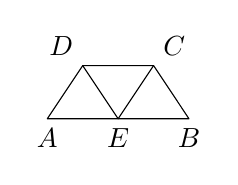
\begin{tikzpicture}[x=0.9cm,y=0.78cm,line cap=round,line join=round]
\coordinate (A) at (0,0); \coordinate (E) at (1,0); \coordinate (B) at (2,0);
\coordinate (D) at (0.5,0.866); \coordinate (C) at (1.5,0.866);
\draw (A)--(D)--(C)--(B)--cycle;
\draw (D)--(E)--(C);
\node[below] at (A) {$A$}; \node[below] at (E) {$E$}; \node[below] at (B) {$B$};
\node[above left] at (D) {$D$}; \node[above right] at (C) {$C$};
\end{tikzpicture}
